\documentclass{article}
\usepackage[top=2.5cm, bottom=2.5cm, left=2cm, right=2cm]{geometry}
\usepackage{amsmath} 
\usepackage{amssymb}
\usepackage{mathrsfs}
\usepackage{amscd}
\usepackage{graphicx} 
\usepackage{subfig} 
\usepackage{tabularx}
\usepackage{indentfirst} 
\usepackage{array}
\usepackage{longtable}
\usepackage{multirow}
\usepackage{bm}
\usepackage{cite}
\usepackage{enumerate}

\author{Wang Dongying}
\title{Outline of Maxwell Equations}
\begin{document}
\maketitle

	The electromagnetic theory of optics begins with Maxwell Equation.

	\section{Maxwell Equations}

		\begin{equation}
		\begin{aligned}
			\nabla\cdot\bm{D} = \rho\\
			\nabla\cdot\bm{B} = 0\\
			\nabla\times\bm{E} = -\frac{\partial\bm{B}}{\partial t}\\
			\nabla\times\bm{H} = \frac{\partial\bm{D}}{\partial t} + \bm{J}
		\end{aligned}
		\end{equation}

	\section{Constitutive Relations}

		$$\bm{D} = \epsilon_{0}\bm{E} + \bm{P} \ \ \ \ \ \ \ \ \ \epsilon_{0} = 8.854 \times 10^{-12}$$
		$$\bm{B} = \mu_{0}\bm{H} + \bm{M} \ \ \ \ \ \ \ \ \ \ \ \mu_{0} = 4\pi \times 10^{-7}$$

	\section{Boundary conditions}

		\begin{equation}
		\begin{aligned}
			E_{1t} - E_{2t} = 0\\
			H_{1t} - H_{2t} = \bm{J}_{s} \times \bm{n}\\
			D_{1n} - D_{2n} = \rho_{s}\\
			B_{1n} - B_{2n} = 0
		\end{aligned}
		\end{equation}

	\section{Charge conservation}

		$$\frac{\partial \rho}{\partial t} + \nabla\cdot\bm{J} = 0\ \ \ \ \ \ \to \ \ \ \ \rho(r,t) = \rho_{0}(r)e^{-\sigma t/\tau}$$

	\section{Energy flux and energy conservation}

		Because energy can be converted into different forms, the corresponding conservation equation should have a non-zero term in the right-hand side corresponding to the rate by which energy is being lost from the fields into other forms.

		\begin{equation}
		\begin{aligned}
			\frac{\partial \rho_{en}}{\partial t} + \nabla\cdot\bm{J}_{en} = rate of energy loss\\
			\rho_{en} = w = \frac{1}{2}\epsilon|E|^{2} + \frac{1}{2}\mu|H|^{2}\\
			\bm{J}_{en} = \bm{S} = \bm{E \times H} \ \ \ \ \ poynting vector\\
			\frac{\partial w}{\partial t} + \nabla\cdot\bm{S} = -\bm{J}_{en}\cdot\bm{E}
		\end{aligned}
		\end{equation}

	\section{Harmonic Time dependence}

		Maxwell’s equations simplify considerably in the case of harmonic time dependence. We assume that all fields have a time dependence $e^{i\omega t}$.

		$$\bm{E}(r,t) = \bm{E}(r)e^{i\omega t}\ \ \ \ \ \ \ \ \ \ \bm{H}(r,t) = \bm{H}(r)e^{i\omega t}$$

		We may rewrite Maxwell Equations in the form

		\begin{equation}
		\begin{aligned}
			\nabla\cdot\bm{D} = \rho\\
			\nabla\cdot\bm{B} = 0\\
			\nabla\times\bm{E} = -i\omega\bm{B}\\
			\nabla\times\bm{H} = i\omega\bm{D} + \bm{J}
		\end{aligned}
		\end{equation}

	\section{Dielectrics}

		A simple model for the dynamics of the displacement x of the bound electron is as follows

		\begin{equation}
			m\ddot{x} = eE - kx - m\gamma\dot{x}
		\end{equation}

		spring-like restoring force to the binding of the electron to nucleus.\\
		friction-type force proportional to the velocity of the electron\\

		\begin{equation}
			\ddot{x} + \gamma\dot{x} + \omega_{0}^{2}x = \frac{e}{m}E
		\end{equation}

		suppose the solution has the form as $x(t) = xe^{i\omega t}$

		\begin{equation}
			-\omega^{2}x + i\omega\gamma x + \omega_{0}^{2}x = \frac{e}{m}E
		\end{equation}

		solution

		\begin{equation}
			x = \frac{\frac{e}{m}E}{\omega_{0}^{2} - \omega^{2} + i\omega\gamma}
		\end{equation}

		the corresponding velocity

		\begin{equation}
			v = \frac{i\omega\frac{e}{m}E}{\omega_{0}^{2} - \omega^{2} + i\omega\gamma}
		\end{equation}

		the effective permittivity

		\begin{equation}
			\epsilon(\omega) = \epsilon_{0} + \frac{\frac{Ne^{2}}{m}}{\omega_{0}^{2} - \omega^{2} + i\omega\gamma} = \epsilon_{0} + \frac{\epsilon_{0}\omega_{p}^{2}}{\omega_{0}^{2} - \omega^{2} + i\omega\gamma}
		\end{equation}

		where $\omega_{p}$ is so-called plasma frequency of material. The real and imaginary parts of $\epsilon(\omega)$ characterize the refractive and absorptive properties of the material. By convention, we define the imaginary part with the negative sign:

		\begin{equation}
		\begin{aligned}
			\epsilon(\omega) = \epsilon_{1}(\omega) - i\epsilon_{2}(\omega)\\
			\epsilon_{1} = \epsilon_{0} + \frac{\epsilon_{0}\omega_{p}^{2}(\omega_{0}^{2} - \omega^{2})}{(\omega_{0}^{2} - \omega^{2})^{2} + \gamma^{2}\omega^{2}} \ \ \ \ \ \ \ \ \ \epsilon_{2} = \frac{\epsilon_{0}\omega_{p}^{2}\omega\gamma}{(\omega_{0}^{2} - \omega^{2})^{2} + \gamma^{2}\omega^{2}}
		\end{aligned}
		\end{equation}

		\begin{figure}
  		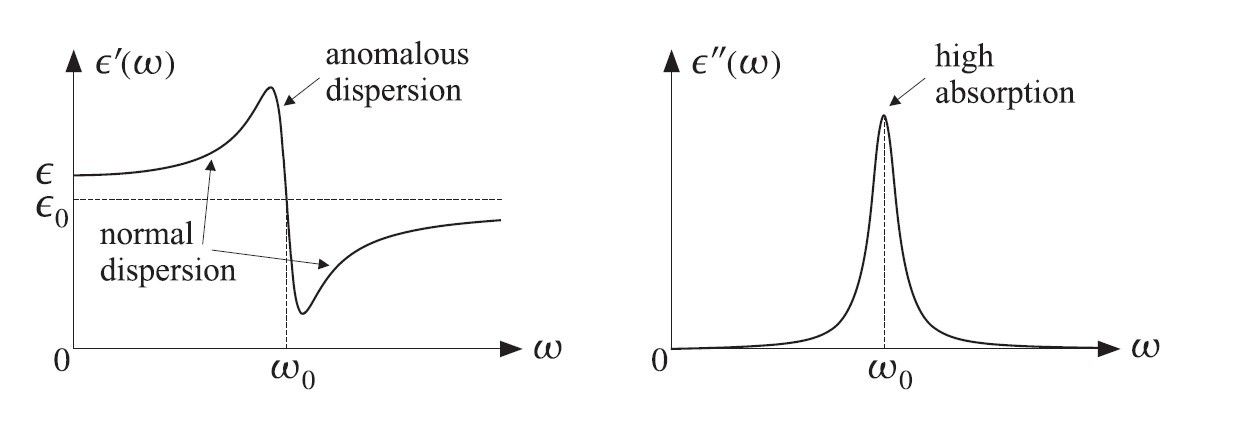
\includegraphics[width=\linewidth]{fig1.jpg}
  		\caption{Real and imaginary parts of the effective permittivity}
		\end{figure}

		Real dielectric materials exhibit serveral such resonant frequency corresponding to various vibrational modes and polarization mechanisms.

		\begin{equation}
			\epsilon(\omega) = \epsilon_{0} + \epsilon_{0}\Sigma_{i}\frac{\frac{N_{i}e_{i}^{2}}{m_{i}\epsilon_{0}}}{\omega_{i}^{2} - \omega^{2} + i\omega\gamma_{i}}
		\end{equation}

		A more correct quantum-mechenical treatment leads essentially to the formula

		\begin{equation}
			\epsilon(\omega) = \epsilon_{0} + \epsilon_{0}\Sigma_{j>i}\frac{\frac{f_{ji}(N_{i} - N_{j})e^{2}}{m\epsilon_{0}}}{\omega_{ji}^{2} - \omega^{2} + i\omega\gamma_{ji}}
		\end{equation}

		where $\omega_{ji}$ is transition frequency, $\omega_{ji} = (E_{j} - E_{i})/\hbar$.

	\section{Conductors}

		The conductivity properties of a material are described by Ohm’s law. Define the conductivity $\sigma(\omega)$.
		\begin{equation}
			J = \rho v = Nev = \frac{i\omega\frac{Ne^{2}}{m}E}{\omega_{0}^{2} - \omega^{2} + i\omega\gamma} = \sigma(\omega)E
		\end{equation}

		This is related to the expression of permittivity.

		\begin{equation}
			\epsilon(\omega) = \epsilon_{0} - i\frac{\sigma(\omega)}{\omega}
		\end{equation}

		Since metal conduction charges are unbound, we take $\omega_{0} = 0$,
		\begin{equation}
			\sigma(\omega) = \frac{\epsilon_{0}\omega_{p}^{2}}{\gamma + i\omega} \ \ \ \ \ (Drude model)
		\end{equation}
		





















\end{document}